\section{Research through Design}

When it comes to the structural nature of the coming-together of this thesis, the methodology, I have followed an approach to research practise called Research through Design (RtD).

This research approach was first coined by \autocite{frayling_1994}, in a highly influential paper where he addressed the debate and confusion at the time around what research \emph{is}, what it \emph{involves}, and what it \emph{delivers}. Frayling critiques the stereotypical perceived difference between the Research field and the Art and Design field - whereas 'researching' stereotypically is seen as a cognitive practise, while art and design is seen as an expressive practise \autocite[p. 5]{frayling_1994}. Concluding that since many of the motivations and practises of the two fields are alike, there is a more productive distinction of the relations between research, art and design \autocite[p. 5]{frayling_1994}, namely: research \emph{into} art and design, research \emph{through} art and design, and research \emph{for} art and design. 

According to Frayling, Research \emph{into} art and design is concerned with historical research, aesthetic and perceptual research, and research into theoretical perspectives on art and design \autocite[p. 5]{frayling_1994}. Research \emph{for} art and design on the other hand is research "where the end product is an artefact - where the thinking is, so to speak, \emph{embodied in the artefact}, where the goal is not communicable knowledge in the sense of verbal communication, but in the sense of visual or iconic or imagistic communication"\autocite[p. 5]{frayling_1994}. Lastly, Research \emph{through} art and design is concerned with either/ or materials research, development work (i.e. customising a piece of technology to do something no-one had considered before, and communicate the results), as well as action research (i.e. where a research diary tells, in a step-by-step way, of the experiment and result), underlining how "both the diary and the report are there to \emph{communicate the results}, which is what separates \emph{research} from the gathering of reference materials" \autocite[p. 5]{frayling_1994}.
\par
\textbf{The thing is, during this thesis project I have only done one 'designing' activity (ref. section 8.3: Exploring input through plants), that would suggest a fit into Frayling's description of research through design, as a type of development work. As I hope will become clear, the main reason for this thesis to be placed into the RtD approach by Frayling, is because the process diary and thesis report as a whole documents the subjective, but theoretically grounded progression I (as a researcher) have gone through in terms of gaining knowledge and understanding as to how one can design meaningful interactive experiences in a museum space that addresses sustainability.
}

In the next section I will go through and describe the "steps" (or "moving") I have taken during the thesis project, and how theoretical practise is weighted against (actual) experiences and critical analysis of a set of interactive exhibitions and installations.


\section{How the thesis have developed over time}

I this section I want to give reason as to why and how the thesis research question have changed 




To begin with, the

\section{Model of interaction design research}
Throughout this thesis project, there has been a major directional shift that has affected the research outcome - something which happened right about in the middle of things. I started this thesis project with a pretty clear goal to prototype and design an installation, but have ended up with a critical study of a number of interactive exhibitions and installations that I analyse to identify meaningful relationships or qualities in a museum space. To better show and talk-through this shift, I will use Fallman's model of interaction design research, which I often refer to as 'the design triangle', to better describe how my researching lens have shifted throughout and during the thesis project. It is also a means to explain as to why and how this thesis is fitted and give back to the interaction design research field.

As a design discipline, interaction design’s core can be found in an orientation towards the shaping of digital artefact, products, services, and spaces - with particular attention paid to the qualities of the user experience \autocite[p. 4]{fallman_triangle_2008}. In Fallman’s use of the model, the most interesting and rewarding results in interaction design research come not from taking a specific position in the model, but rather from moving or drifting in between different positions. Thus, as Fallman describe it, "moving in between different positions in the model is, more than anything else, a change of perspective" \autocite[p. 10]{fallman_triangle_2008}.


\begin{figure}[H]
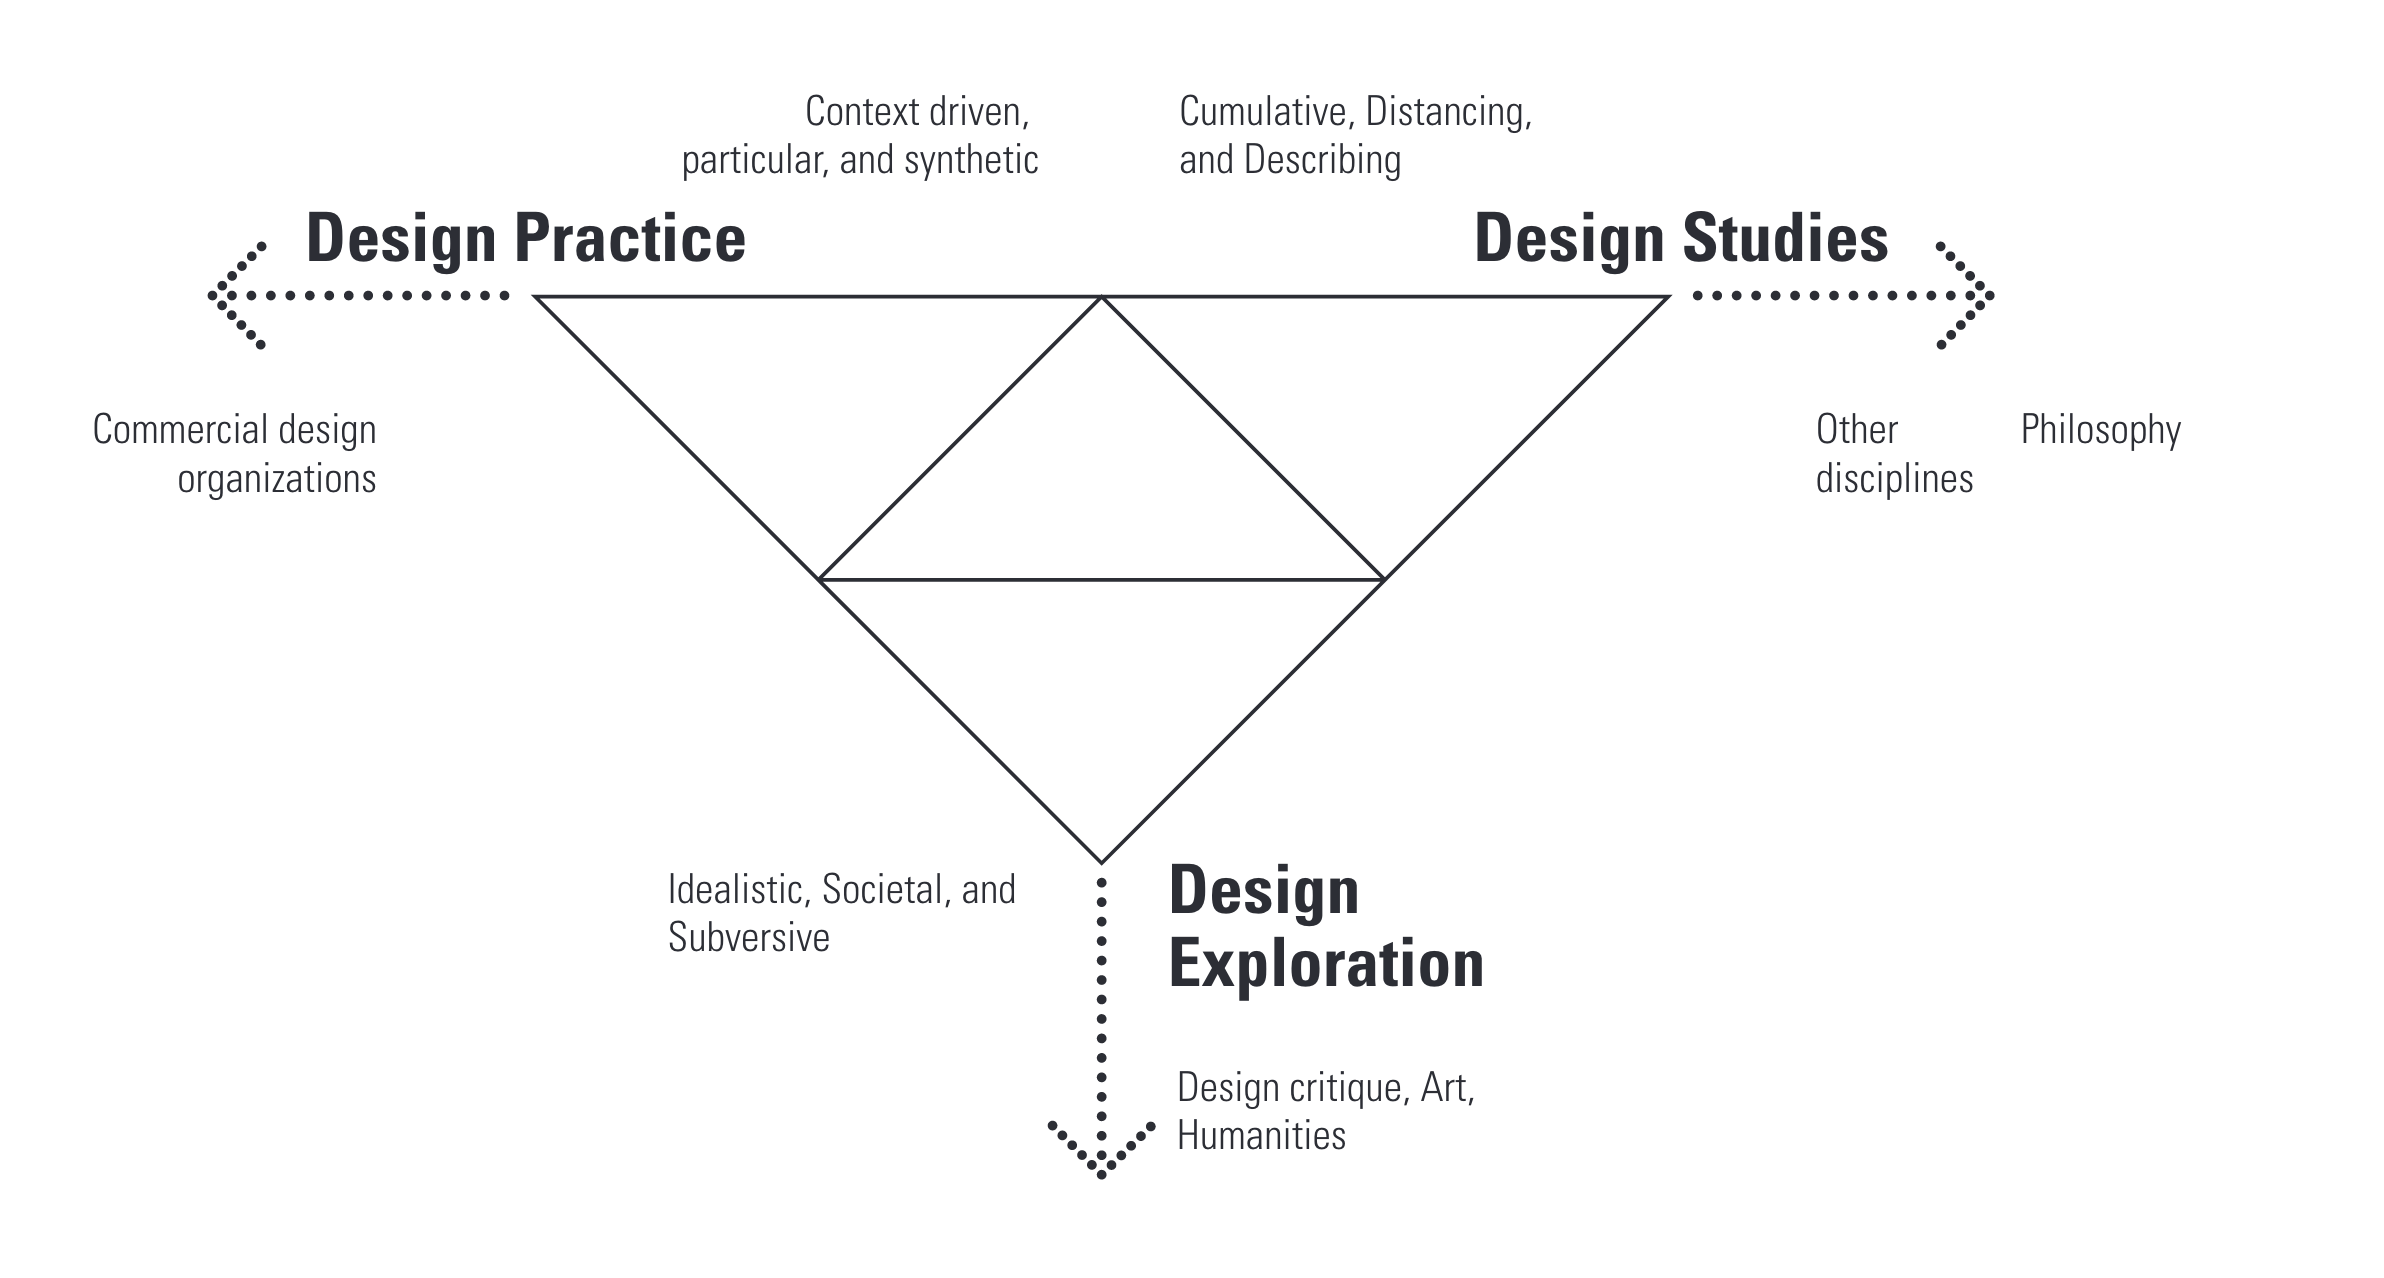
\includegraphics[width=13cm]{pictures/process/triangle.png}
\caption{"The model of interaction design research in its most basic form."}
\autocite[p. 5]{fallman_triangle_2008}
\centering 
\end{figure}

% In terms of doing research through design as a method for interaction design, Zimmerman et. al, explains that what is unique to research though design as an approach, is that it sees the design artefacts as outcomes that can transform the world from its current state to preferred state, which aligns with the domain problems I have accounted for in section 2.0, to address sustainability issues for a more sustainable future. Zimmermann et. al. further explain how the artefacts produced in this type of research become design examples, providing an appropriate channel for research findings to easily transfer to the HCI research and practise communities(Zimmermann et. al, p. 1, 2007).


Design study entails making space for reflections in some kind of structured way on one’s activities: organising reading circles and seminars; and opening up arenas for theoretical, methodological, and philosophical discussions to take place \autocite[p. 18]{fallman_triangle_2008}. The way I have gone forward with this, is to read up on museum practise as evident in chapter 1: Museums, as well as on the topic of sustainability, linking the museum practise up against sustainability. Specifically looking at how sustainability represents a contemporary discourse, and discussing this in relation to how museums want to address and disseminate more contemporary issues to stay relevant. 

+ Design exploration
+ Design Practise


\section{Qualitative research (very unfinished!)}
jeg gjør kritisk forskning: critical design of existing artifacts instead of designing my own. To proper explore Rq I would need t omake a lot of designs, not enough time, better to lean on theory and explore existing installations so that I can actually explore more of them and "talk back to theory". I use theory to analyse installations installations with a design perspective: user experience (meaningful) and dialogical interactive elements/ qualities. 

The paper offers theoretical support for research through design (RtD) by arguing that to legitimise and make use of research through design as \emph{research}, HCI researchers need to explore and clarify how RtD objects contribute to knowledge \autocite[p.2093]{bardzell_immodest_2015}.


Along these lines, Bardzell et.al argue that while the \emph{intentions} of the object's designer are important and annotations are a good mechanism to articulate them, the critical reception of objects can be equally generative of RtD's knowledge impacts \autocite[p. 2093]{bardzell_immodest_2015}.

Bardzell et.al. investigate RtD in its relation to the production of knowledge; specifically, \emph{how design objects are knowledge producers both for those that encounter them and those that design them} \autocite[p. 2093]{bardzell_immodest_2015}. 

To explore how a detailed critique might work when we understand objects as knowledge producers offering to the viewer the possibility to engage in meaning-making practises unfolding a range of complex and multi-faceted views, Bardzell et. al offer a multilevel analysis of a critical design fiction. \autocite[p. 2094]{bardzell_immodest_2015}.

As a field, HCI must answer what sorts of knowledge outcomes can come from objects in (art and) design projects; if we cant, we cannot legitimize RtD as a way of doing HCI research.

My knowledge outcomes from this thesis project:
\begin{itemize}
    \item Proposal of a theoretical lens to read and understand a interactive installations in the museum/ an exhibition. To identify meaningful relations between the dissemination and exhibition practise.
    \item A critical view on the topic of interactivity addressing contemporary topics/issues in a museum space
    \item 
\end{itemize}

This research practise in this thesis is built upon qualitative data through qualitative methods. 

"ethnographic methods" in this thesis: observation, photographic work, interview, conversations, and thinking. 

this thesis has by no means been structured in a read-collect-write linear type of structure.. 

detached researcher? 
What have I been looking for?

Pure subject, what/ who is my subject-object of study?

\section{Joint forces with two research buddies}
It should also be mentioned that a lot of the data collected for this thesis is done along with two other students, which I often refer to as my research buddies. We all chose the same thesis outline, but writes separately and have developed our own research agendas. In the early stages we worked together in terms of getting to know the domain and context, for the most part discussing and sharing literature insights. Eventually, we started to single out different areas of interest and 

\section{Collaborating partner Klimahuset}

The collaboration with Klimahuset and its stakeholders are possible because it is a part of University of Oslo: the Natural History Museum. The museum itself is located in the Botanical Garden at Tøyen, Oslo. Klimahuset represents the type of space where discourses on sustainability matters can take place, available to citizens as a museum. The museum itself is newly opened, particularly aimed at young adults aged 14-16. It will be the main space where me and my research buddies will conduct research activities and investigate sustainability issues such as Earth’s climate systems, consequences of global warming, solutions, and what actions individuals can do to contribute to a sustainable transition and future. An important note to the collaboration is that even though some research activities is conducted at Klimahuset, and the end-exhibition will take place there, the end-installation is not supposed to be an artefact designed for Klimahuset. Klimahuset simply provides the contextual space for learning and discussing sustainability-related topics.


\section{Timeline of events}
In this section I will account for the project timeline, giving an overall summary of the big events that make up the project. Me and my research buddies have conducted all events (data-gathering) together, except for the Workshop in December 2021. Details on each event will be provided in chapter 8: Process. 

The thesis project has been conducted over the course of three semesters. January to June spring 2021 were for the most part theoretical and focused on reading up and getting to know the museum domain, as well as working on synthesising my research area of interest and formulating a research question. Through my supervisor, me and my research buddies initiated contact with Klimahuset, where we were requested to host a workshop in May, and later on do a presentation in June. Next semester, August to December fall 2021, is where most of the practical research efforts were conducted. In September, both me and my research buddies participated in a course about tangible interaction. Through this course we were a part of a team who conceptualised, designed and exhibited an interactive installation during the course duration of one month. Then comes November, where me and my research buddies decided to go to different museums who exhibited interactive installations to experience, observe and collect data on different installations. Late December 2021, my tangible interaction group were requested to exhibit our installation for a group of first-year master students interested in writing about energy-visualisation. And then comes Spring 2022, where the main focus is writing up the thesis. In February we were given the opportunity to observe two school-classes in Klimahsuet, and given a little time to interview with the working Docent's - which we accepted. In March, our supervisor reached out to the Munch museum and giving us the opportunity to interview a concept developer, which we also accepted. I have drawn up a timeline showing the events throughout the three semesters:

\begin{figure}[H]
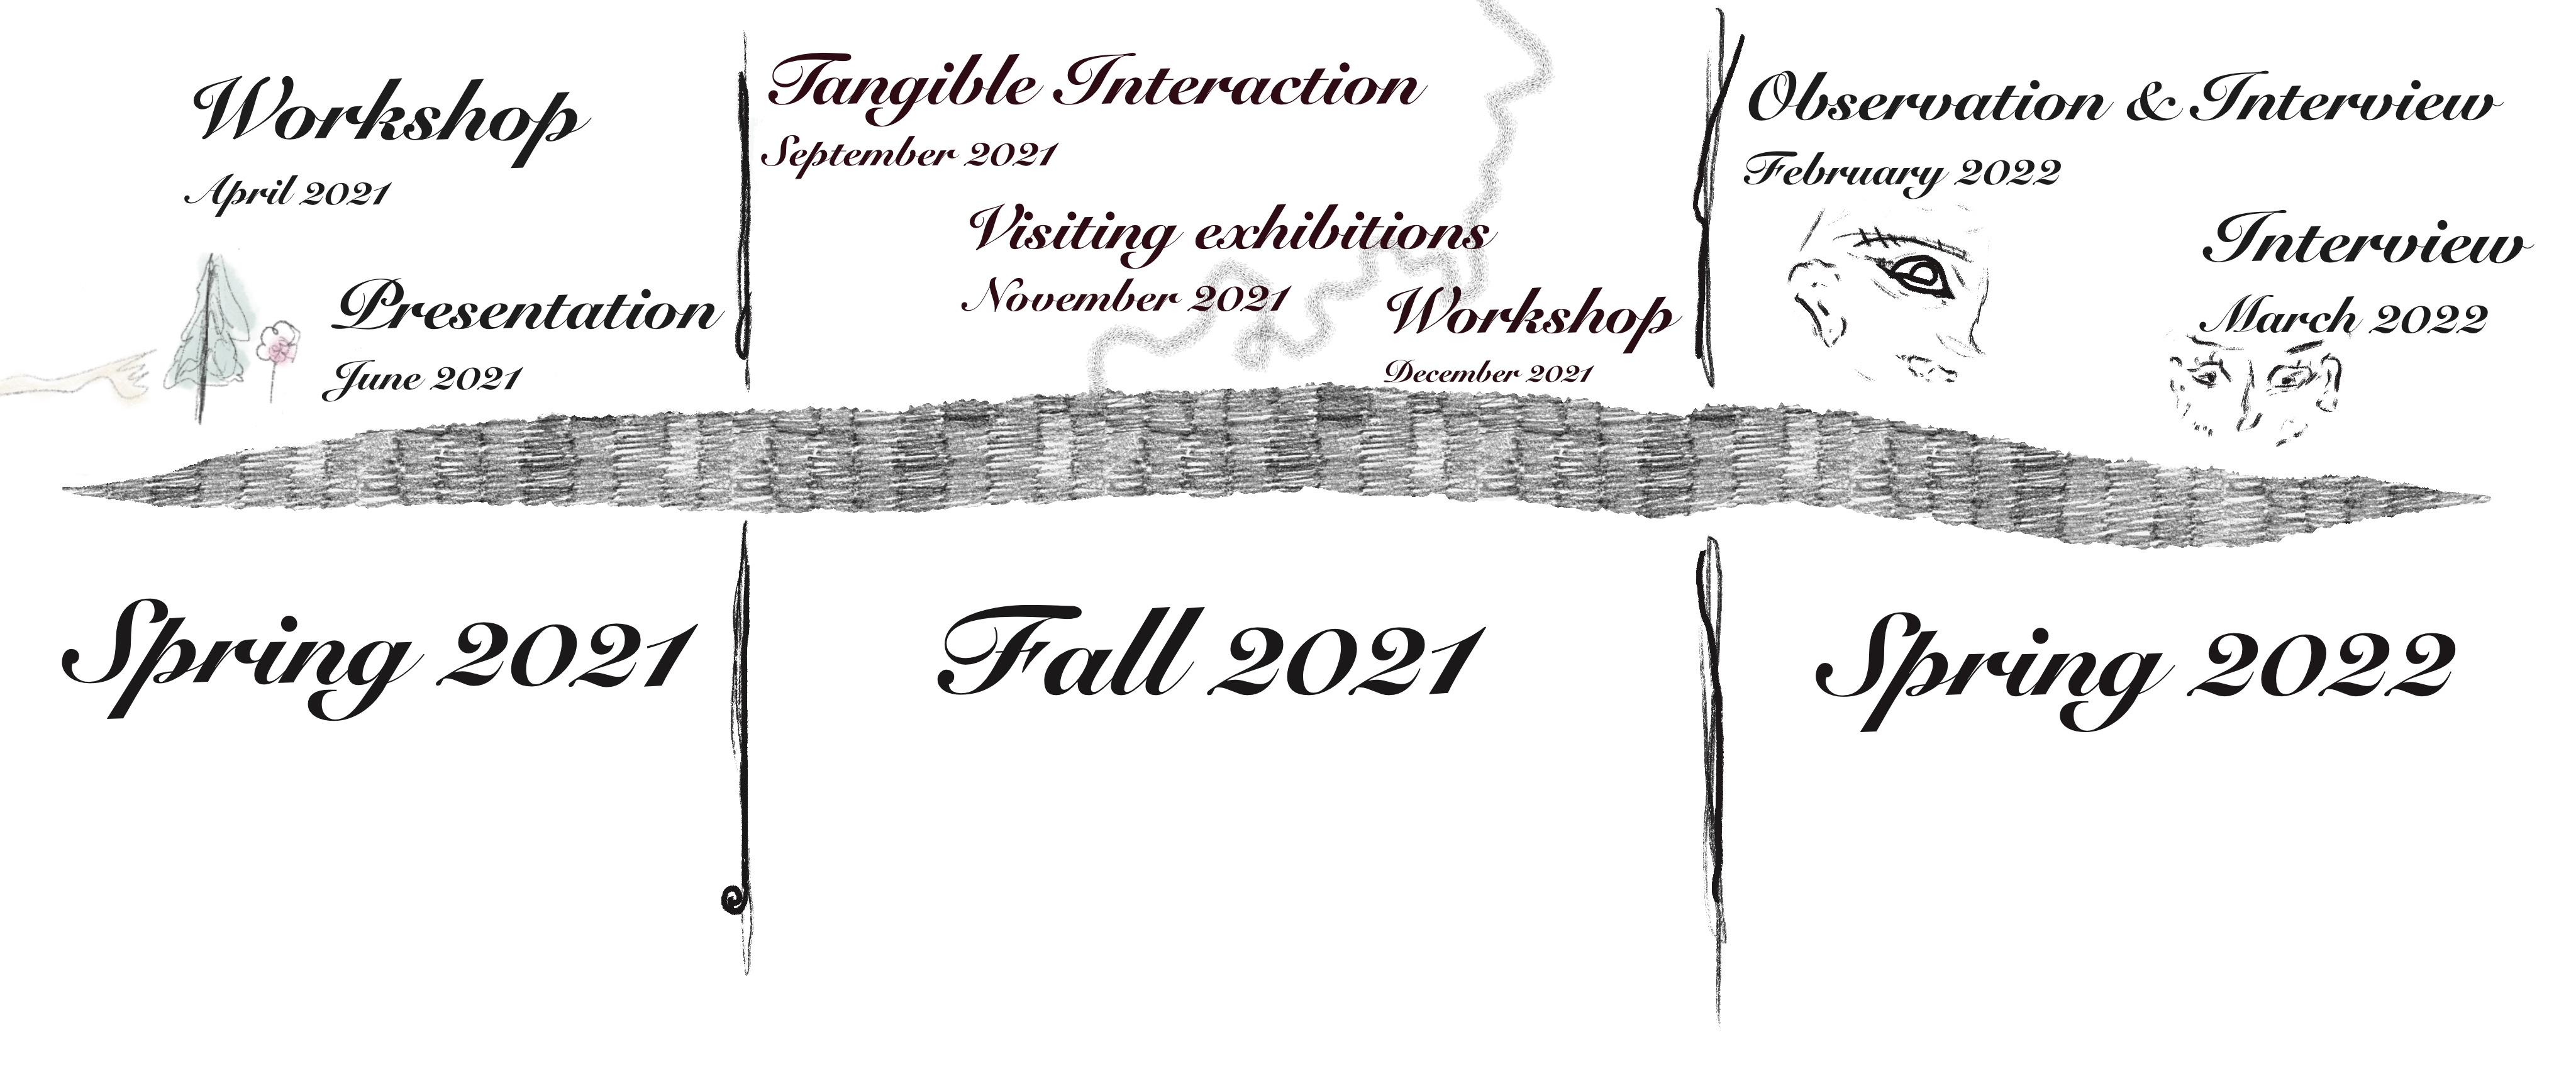
\includegraphics[width=14cm]{pictures/timeline.jpg}
\caption{Timeline of research events}
\centering 
\end{figure}


\section{The dataset}
Over the course of this thesis, my research buddies and I have visited in total 10 exhibitions from 7 different museums in Oslo. From these museum visits, we have documented 22 interactive installations that forms the dataset used for analysis and similar investigations in our respective thesis's. 

\begin{itemize}
    \item Workshop with stakeholders from Klimahuset, april 21
    \item Presentation w/ prototypes at Klimahuset, june 21
    \item Visited 5 different interactive exhibitions, fall 21
    \item Energy visualisation workshop with Qi-installation
    \item Observation of 2 school children classes in Klimahuset, february 22
    \item Interview with two of Klimahuset Docents, february 22
    \item Interview and observation w/ concept developer at Munch, march 22
    \item Analysis/ theorethical framework workshop sessions
\end{itemize}

\begin{figure}[H]
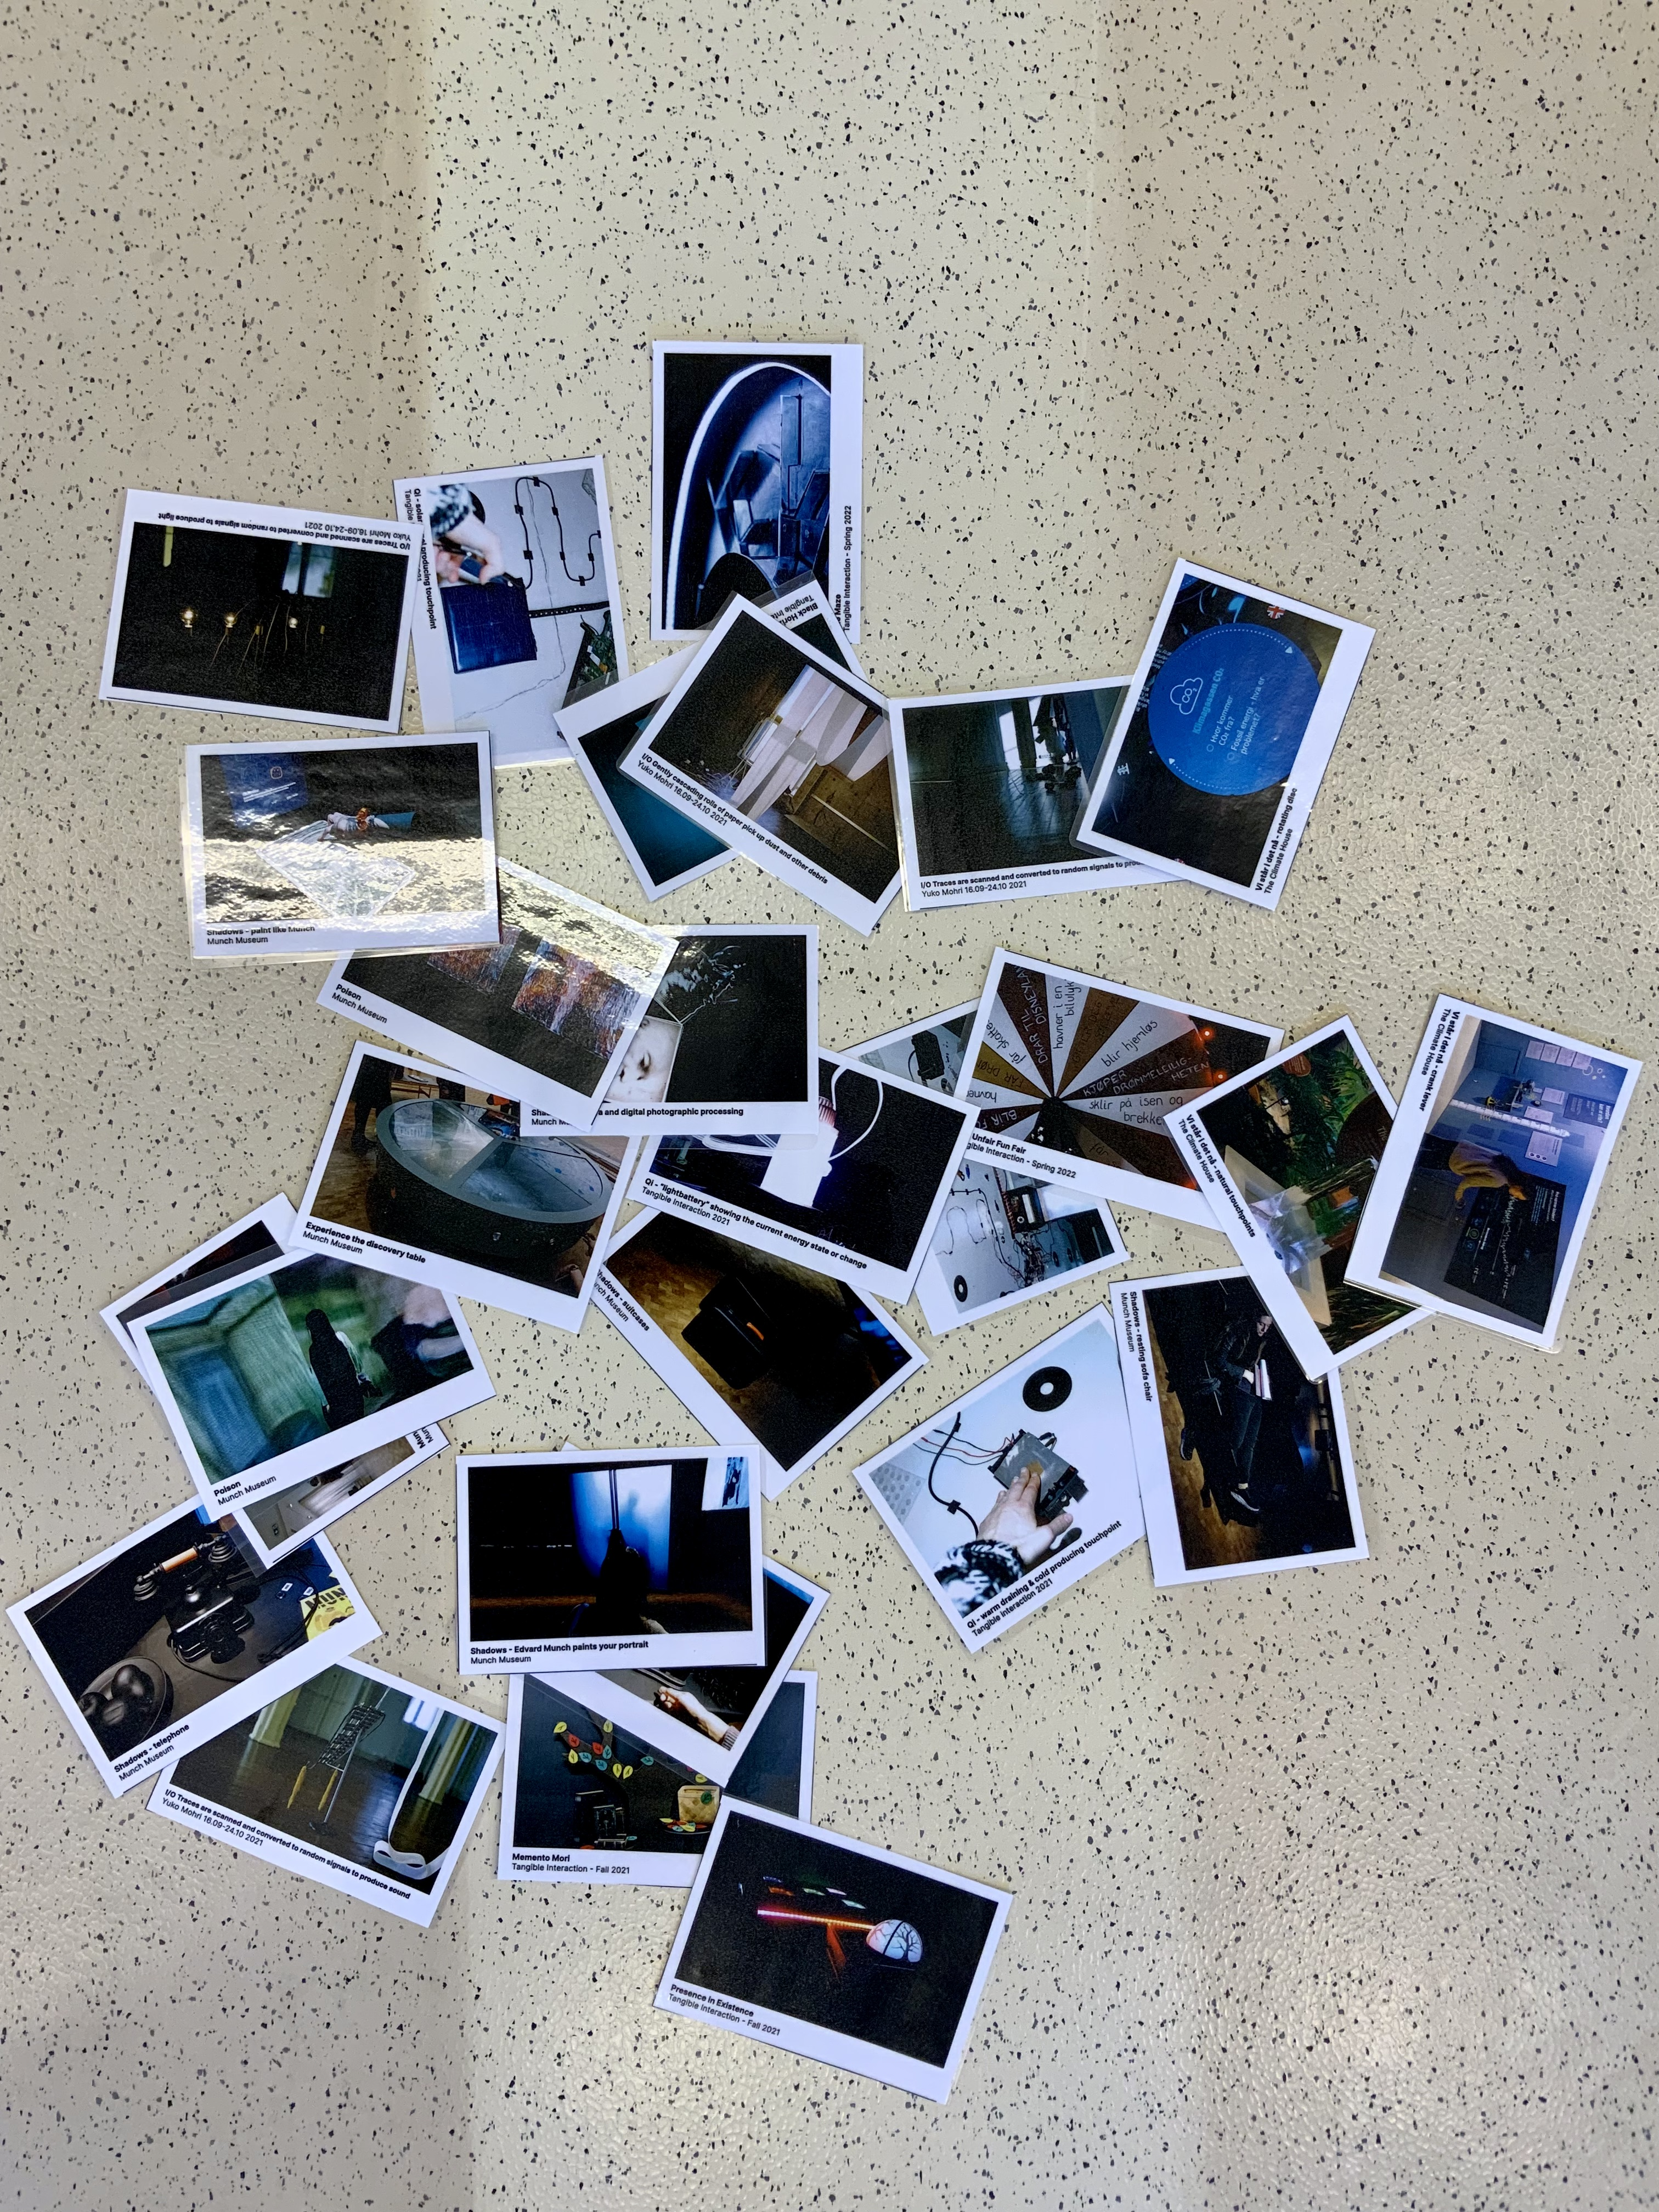
\includegraphics[width=12cm]{pictures/dataset/datasett_oversikt.jpeg}
\centering 
\end{figure}

I think this is basic qualitative analysis?

Måten jeg har gått frem på ved bruk av dette datasettet, sett opp mot mine utvalgte teorier, har vært en form for deduktiv systematisk prosess. Det vil si at jeg til å begynne med har systematisert og kategorisert installasjonene opp mot hver teori; feks som jeg har gjort her fra en av de interaktive installasjonene på klimahuset haar jeg

\subsection{"data laundering"}
Write out:
\begin{itemize}
    \item explain why munch shadows is analysed as one. and only weighted as one. and how that affects the dataset.
    \item discuss how the amount of tangible installations affect the dataset
    \item discuss the analog-tangible vs interactive-tangible installations (ice cube, munch peepholes and discovery table)
\end{itemize}

\begin{figure}[H]
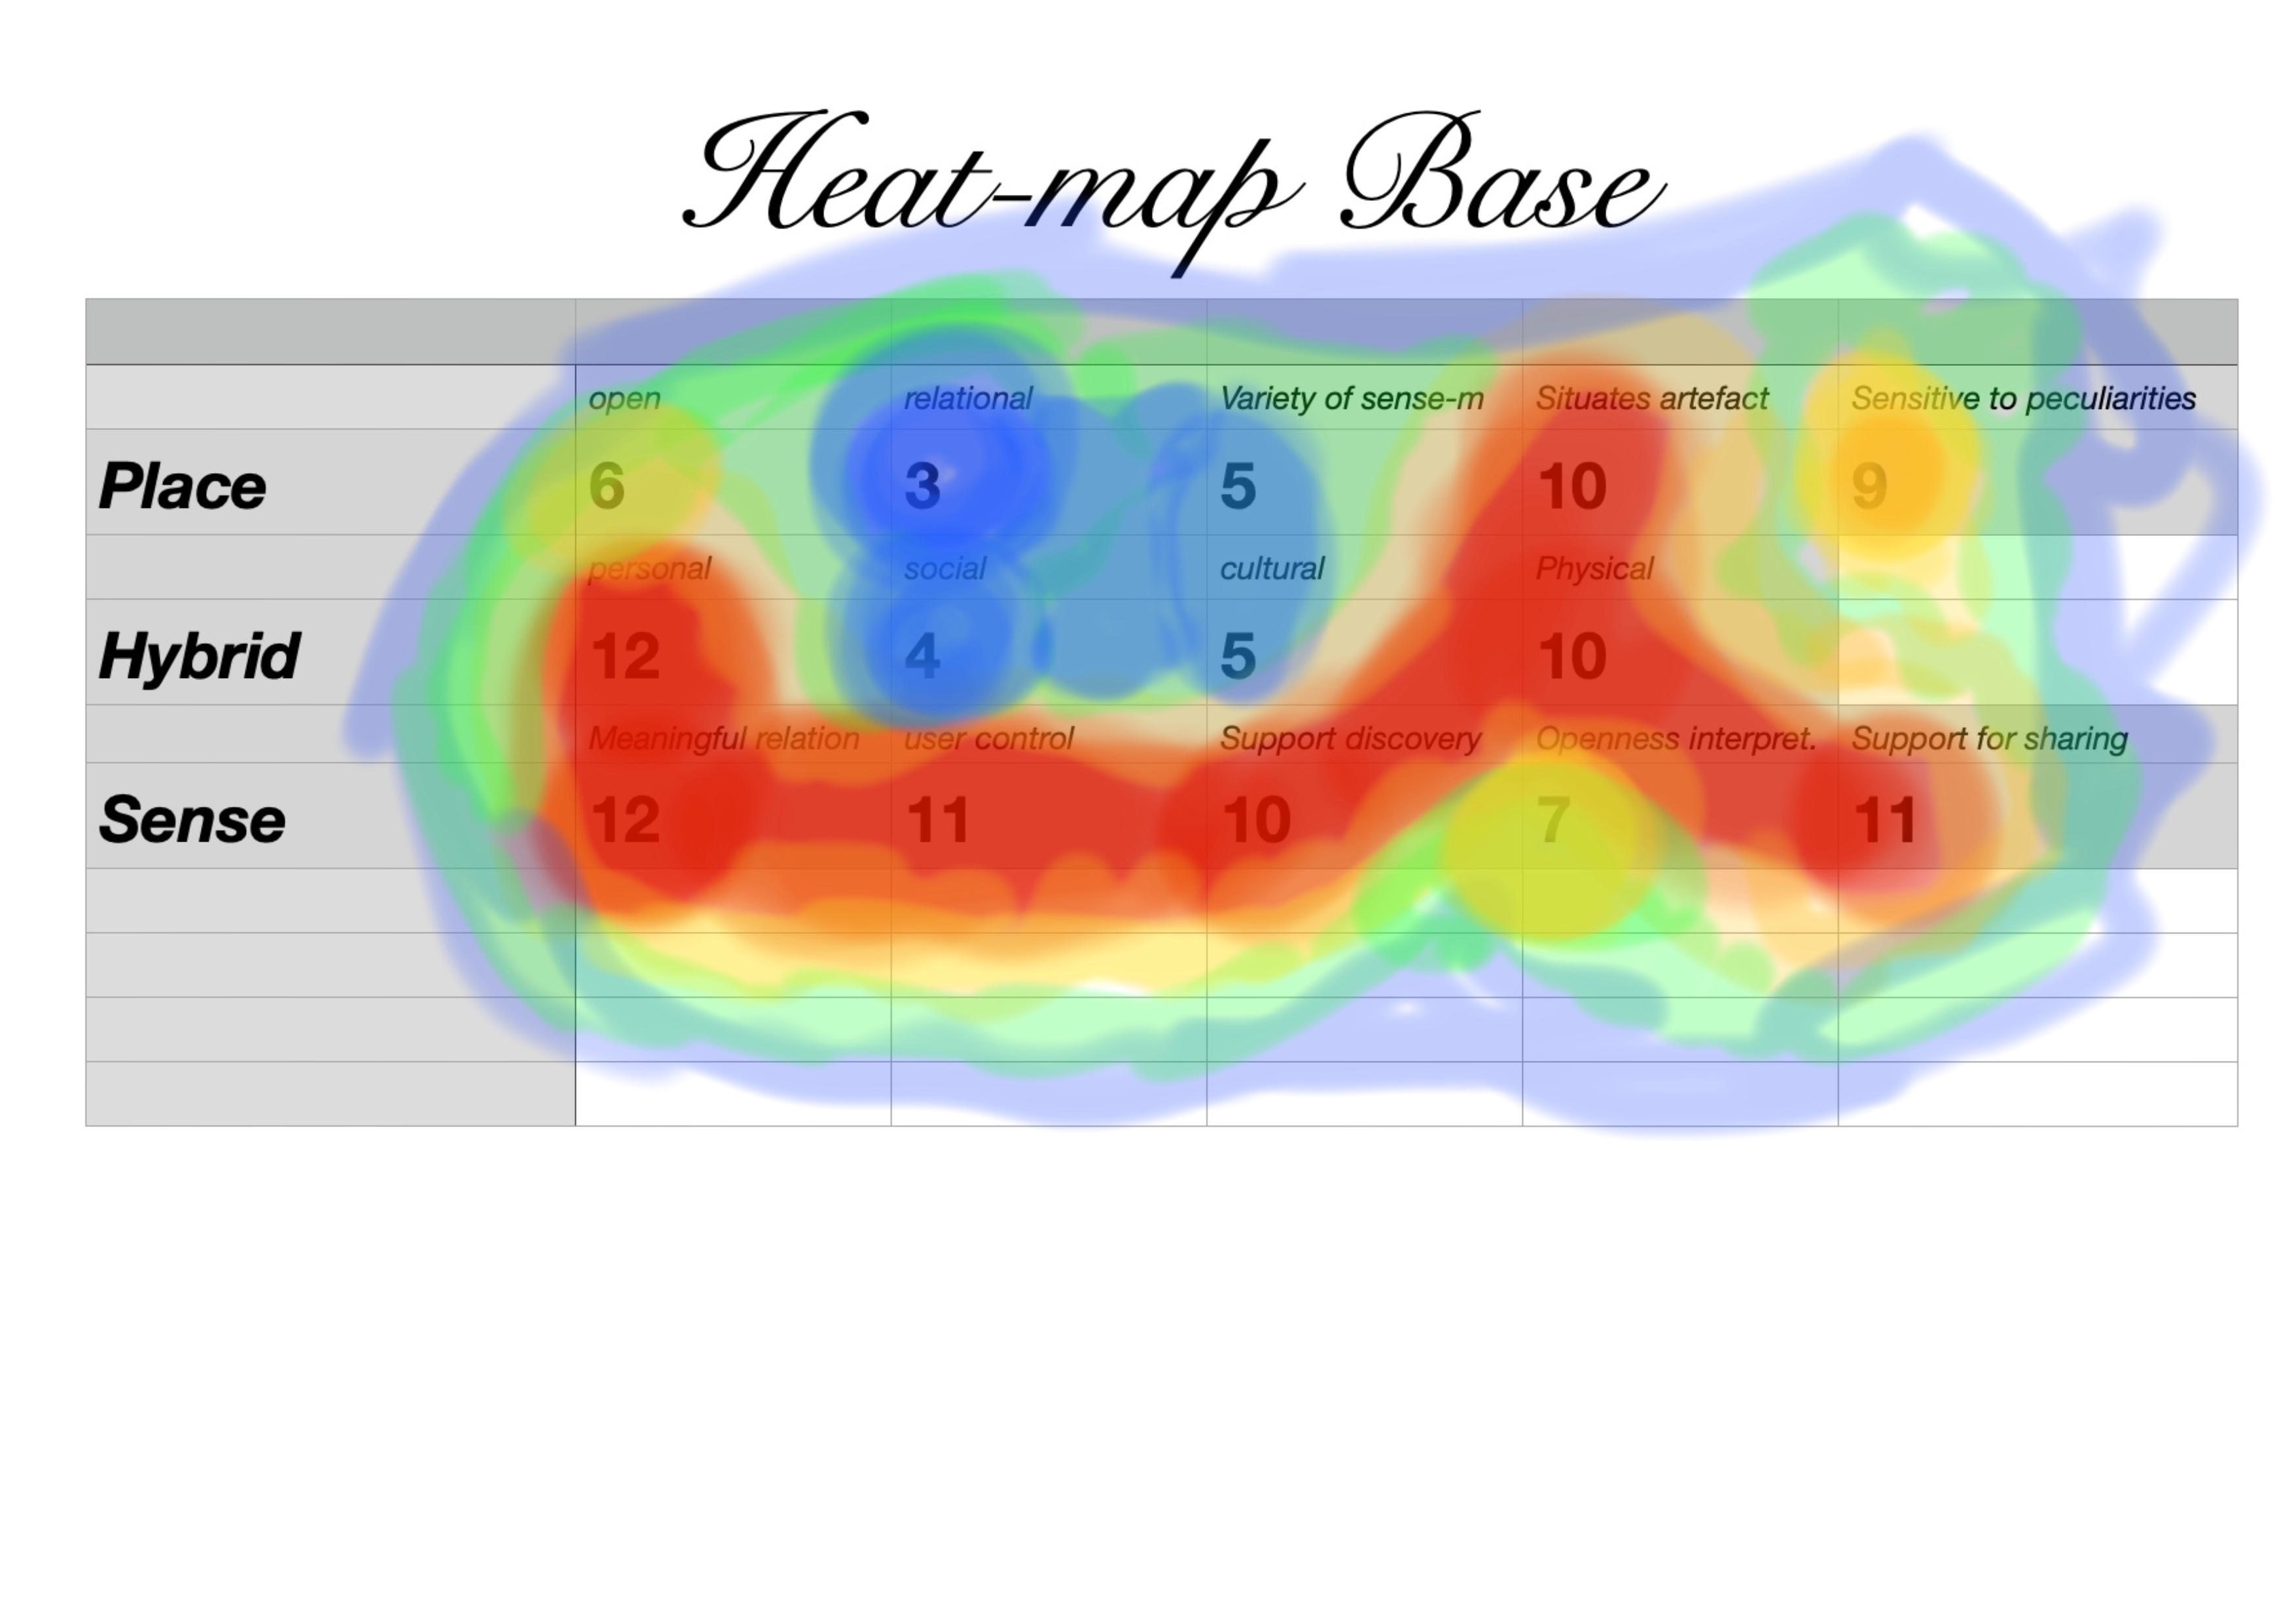
\includegraphics[width=11cm]{pictures/dataset/heatmap.jpg}
\centering 
\end{figure}


\section{First iteration: seeing the bigger picture}

I started the first analytical iteration by sorting the dataset into the three theories I base my understanding of meaningfulness on; \emph{Hybrid place, place as a dialogue} and \emph{Sense-making strategies}. I made one table for each theory, where the frameworks's principles/ and dimensions formed the columns and the 22 different installations the rows. I then went through each installation and plotted in whether or not the installation fulfilled the principle/ dimension. Categorising it this way opened up for looking at the dataset in correlation with each theory separately, making it possible to see overall trends in the dataset according to the theories. Another


respective theory from a birds-eye, holistic, perspective, but it will also work as a quick-reference guide for the second analysis iteration when I'm trying to merge the three theories and/ or finding new relationships between the data across the theories.

The categorisation of the data is highly subjective, but theoretically grounded, based on my personal experience with- and interpretation of the installations and knowledge of the museum institution the installation was part of. I have also chosen to merge all the Munch - \emph{Shadows} installations as one, because they are a part of the same exhibition and do not differ in their interactive qualities. Because of this, the dataset used for this analysis shrinked from 22 to 16. This choice of merging the \emph{Shadows} installations was made in the process of fitting the installations into the theory's principles/ dimensions, when I saw that they all checked the same boxes. 


\begin{figure}[H]
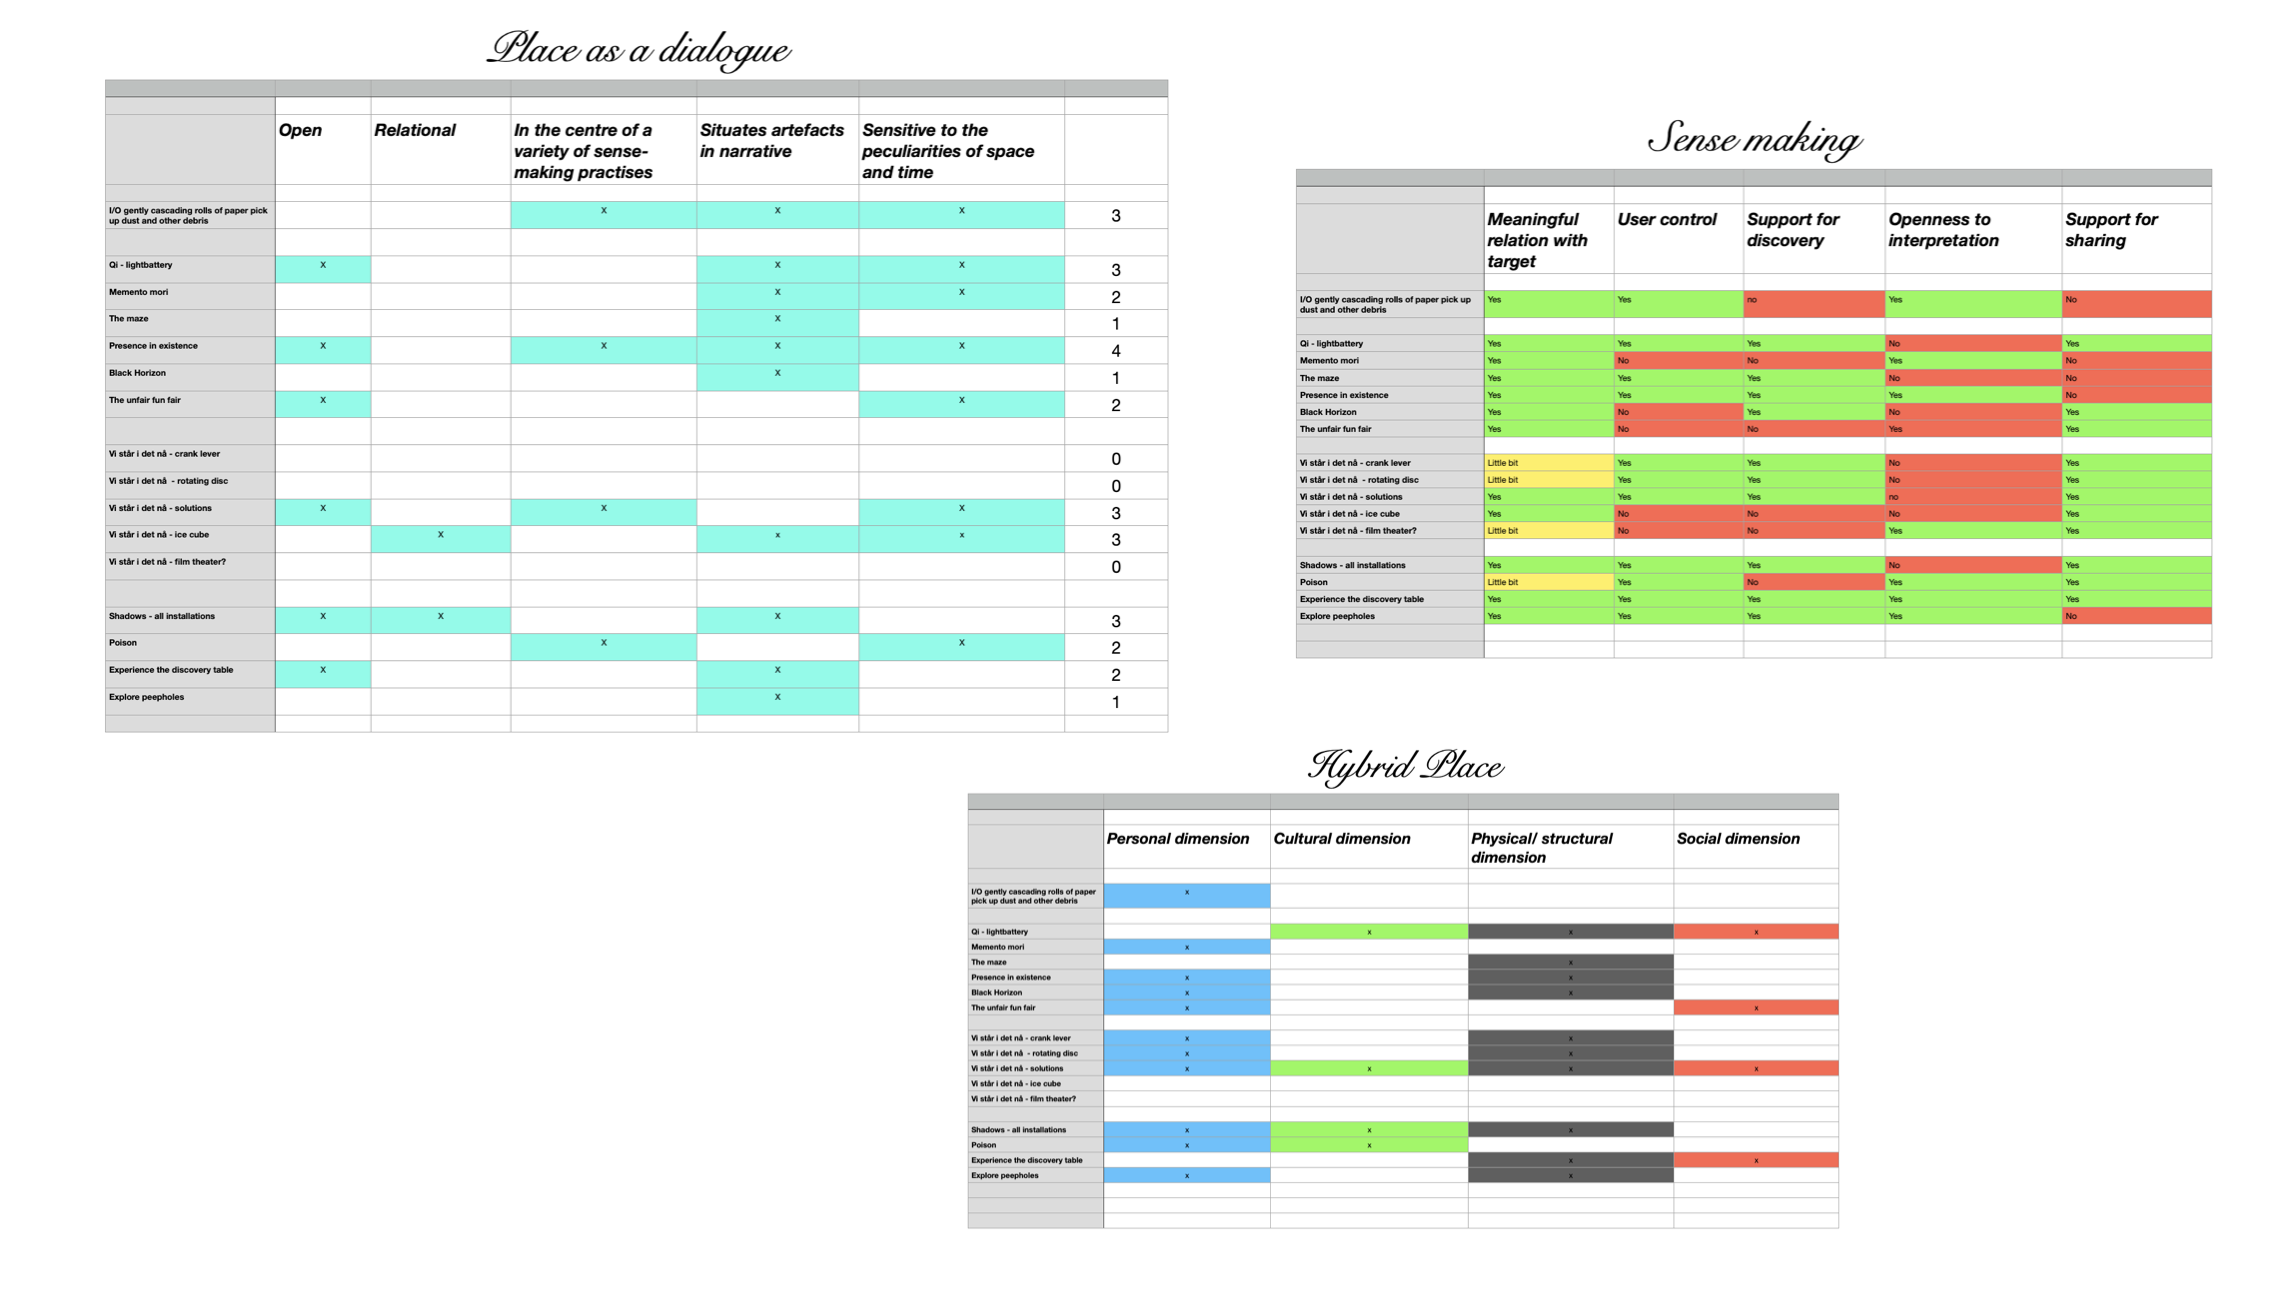
\includegraphics[width=13cm]{pictures/dataset/analysis_tables.png}
\centering 
\end{figure}

After mapping the installations in the tables, it opened up for crunching the first numbers. In this iteration I want to see the dataset from a holistic view. Abstracting from the details and seeing how the installations map up in the bigger picture. To do this I needed a diagram that could compare the different principles up against eachother. I chose to create radar charts to do this, and made a radar chart for each theory. 

\begin{figure}[H]
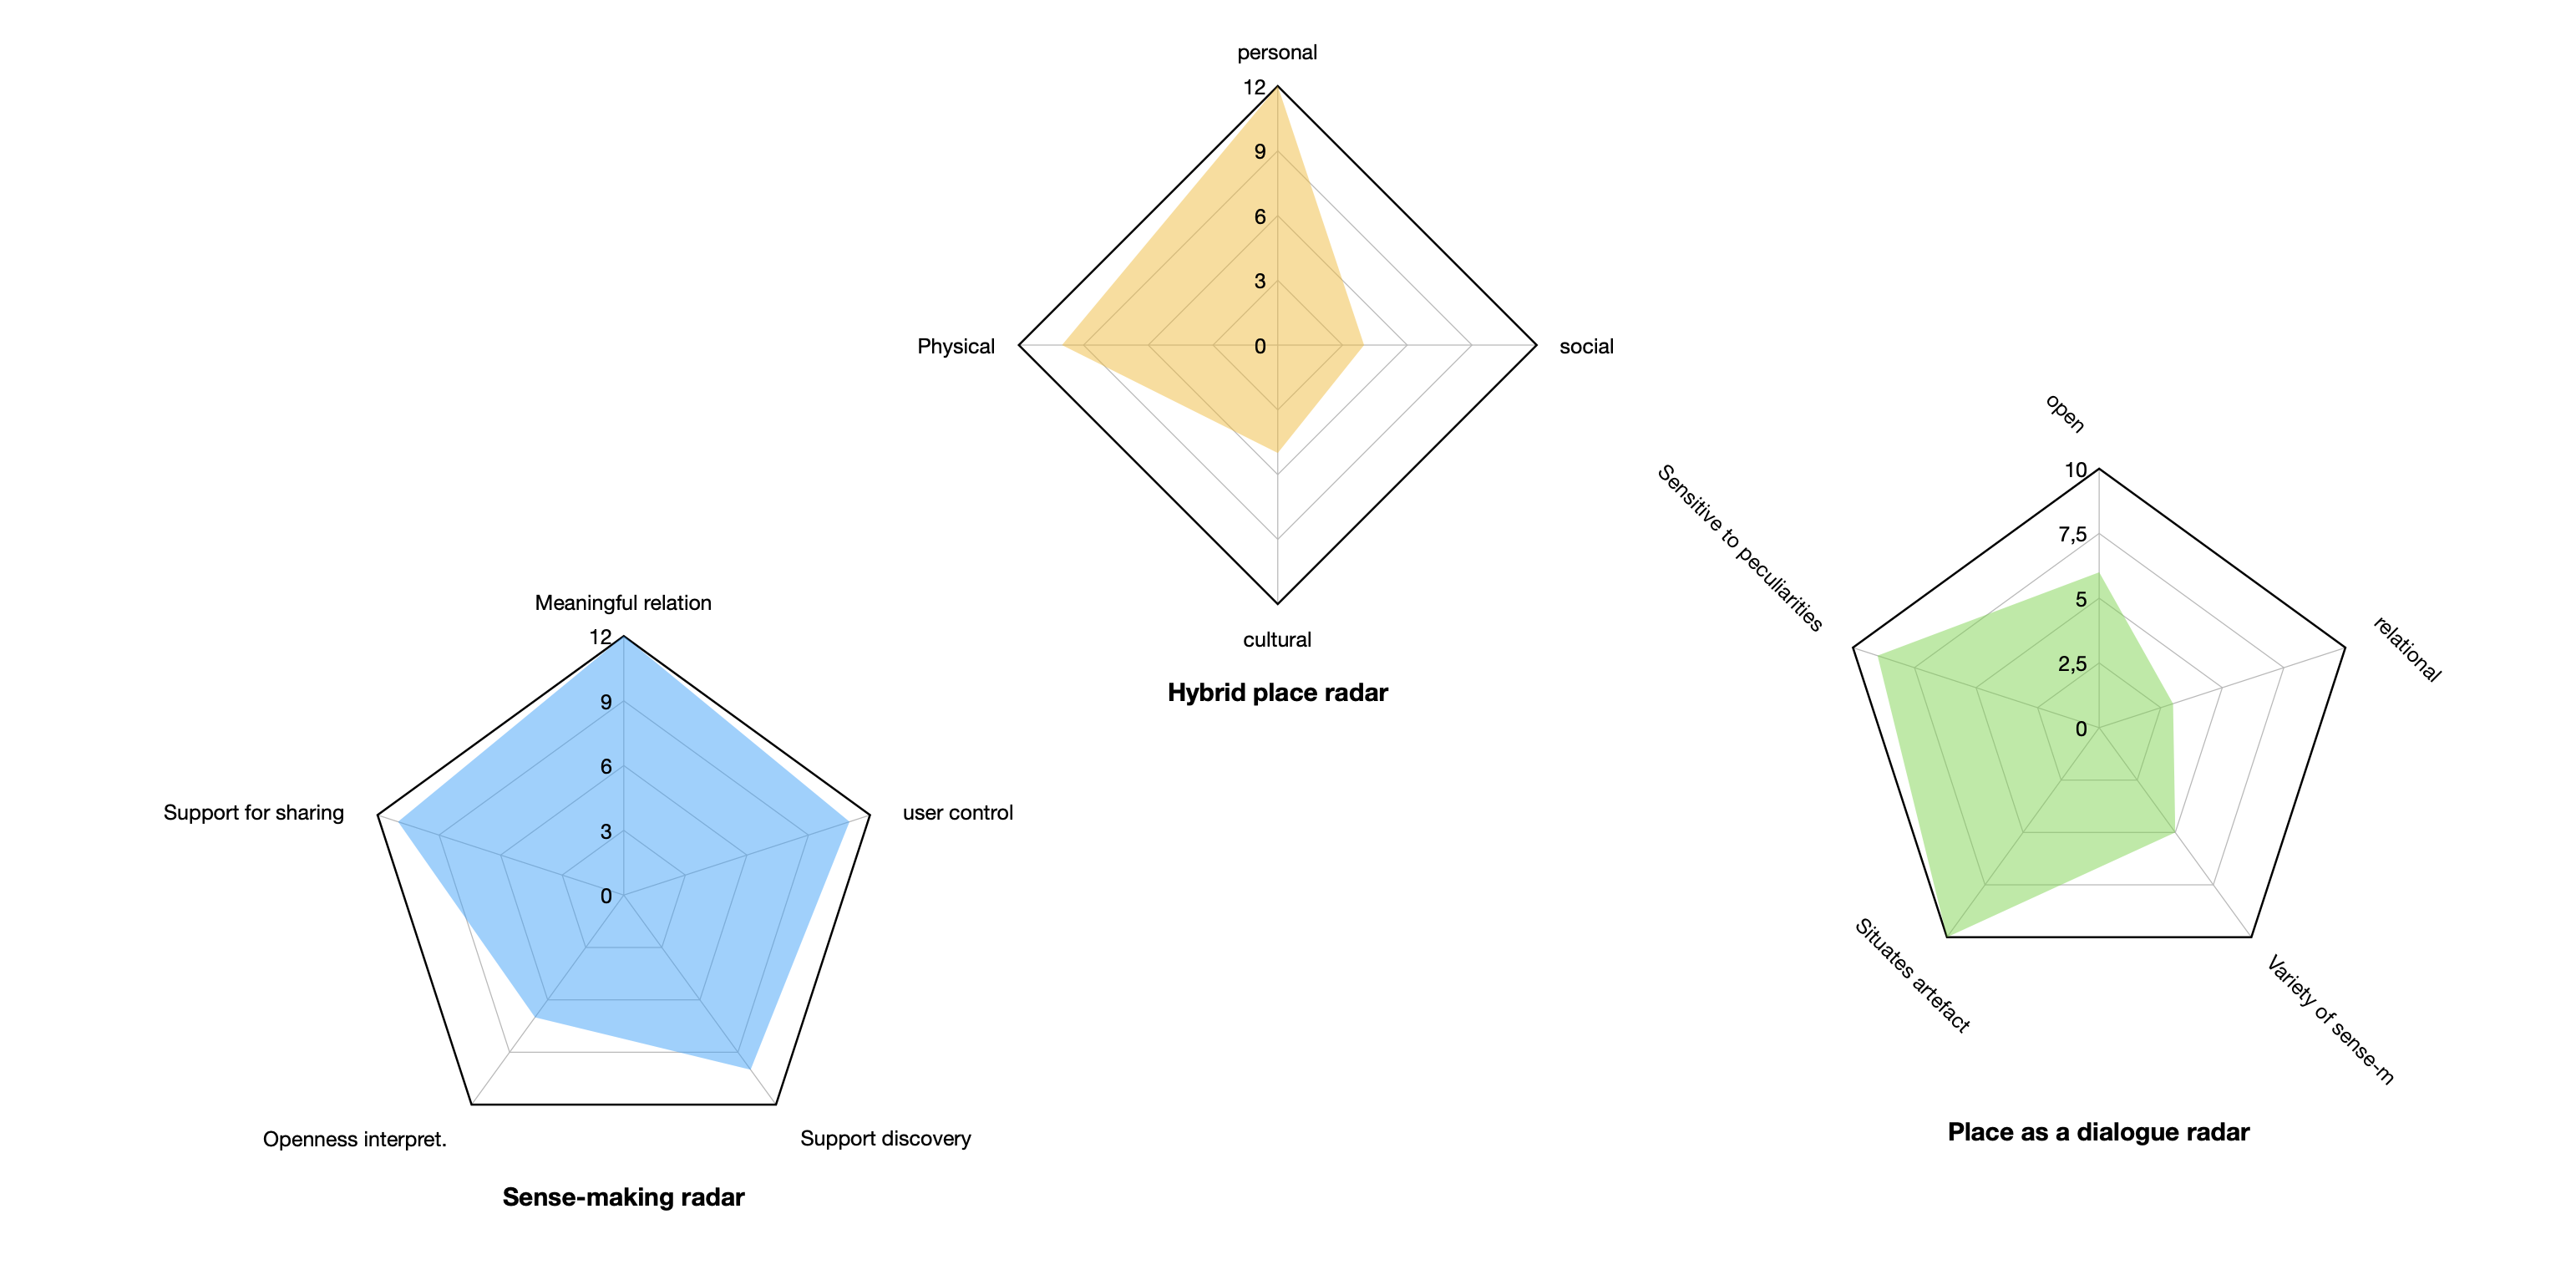
\includegraphics[width=13cm]{pictures/dataset/analysis_radars.png}
\centering 
\end{figure}

\emph{"Findings"}
\par

What I have learned by looking at the radar charts so far is how the different theories fulfill, or complement eachother. The way I have gone forward in looking at the radar charts is as following:
\par I'll start by looking at the hybrid place radar chart, noticing how the personal and physical dimension is fulfilled, while the social and cultural dimension is very little fulfilled. What does this mean? According to the Norwegian museum policy strategic thinking, it is wanted that museums transition from the personal dimension to the more social and cultural dimension. The fact that installations in my analysis shows presence in the physical dimension is positive, in terms of enabling the personal dimension, experience-wise, to involve more tangible or at least dynamic experiences in the museum space.
\par Then, if we shift focus for a second to look into the sense-making radar chart, we see that one of the corners that is fulfilled by almost all installations in this analysis - support for sharing is fulfilled. How come, that even though the social dimension is not fulfilled while almost all installations, in terms of sense-making have good support for sharing? 

\par Then again, we can look at what dialogic qualities the installations turns out to have little "relationalness", which is a dialogic principle/ quality that involves the Docents in the museum for example, or relational qualitites.


\section{Second iteration: Understanding Klimahuset's digital and analog relationships}

hhmmmmmm

\section{The role of prototyping in this thesis (unfinished)}
\autocite[p. 1]{lim_anatomy_2008}
Research through design is a type of research practise where the researcher create artefact- or object prototypes to gain the necessary insight needed to drive and conduct the research project. Prototyping, or the use of prototypes can be used in a variety of ways, and in every stage throughout the project. In the field of human-computer interaction (HCI), software engineering and design, the term prototype is commonly used to signify a specific kind of object used in the design process (Lim et. al., 2008, p. 2). The prototypes are either physical or digital, and function as either a speculative solution, as a manifestation of a design idea, or to explore a design space - all in relation to the research scope and focus. Prototypes are the means by which designers organically and evolutionary learn, discover, generate and refine designs \cite{lim_anatomy_2008, p.2}. They are design-thinking enablers deeply embedded and immersed in design practise, not just as tools for evaluating or proving successes or failures of design outcomes (Lim et. al., 2008, p. 2). 

In the search for a new way of thinking about prototypes and prototyping, based on the need for exploring and establishing a definition that differs from current approaches in software engineering contexts where engineers use prototypes to identify or satisfy requirements: Lim et. al., conceptualise prototypes as tools for traversing a design space where all possible design alternatives and their rationales can be explored (Lim et. al., 2008, p. 2). In that way, the prototype serves as a communicative manifestation, where the designer is enabled to communicate the rationales of their design decisions through the prototype (Lim et. al., 2008, p. 2). Prototypes stimulate reflections, and designers use them to frame, refine and discover possibilities in a design space (Lim et. al., 2008, p. 2). This new way of thinking about prototypes differs markedly from requirement-oriented approaches like software engineering, recognising design activities as flexible rather than rigid, reflective rather than prescriptive, and problem-setting rather than problem-solving (Schön, 1982). A design idea that satisfies all the identified requirements does not guarantee that it is the best design since a number of ways can meet each requirement (Lim et. al., 2008, p. 2). If the focus of prototyping is framing and exploring a design space, what matters is not identifying or satisfying requirements using prototypes but finding the manifestation that in its simplest form, filters the qualities in which designers are interested, without distorting the understanding of the whole (Lim et. al., 2008, p. 2). In order to support this perspective and to provide a stable foundation for the study of prototypes in HCI, Lim et. al. (2008) proposes a framework for conceptualising prototypes. The framework is an attempt to create an understanding of the nature of prototypes in general and to provide a language for articulating the characteristics of a particular prototype (Lim et. al., 2008, p. 3). Two fundamental aspects of prototyping form the basis of the framework:

1) prototypes are for traversing a design space, leading to the creation of meaningful knowledge about the final design as envisioned in the process of design, and
2) prototypes are purposefully formed manifestations of design ideas.
(Lim et. al., 2008, p. 3)

Will answer these:
What values are important in my context?
What is my design outcomes?
What is my design space?
Experience prototyping? Am I going to prototype an experience?
Why and how do I intend a particular prototype to support the design process?